
\documentclass[a4paper]{article}

\usepackage{graphicx}
\usepackage{listings}
\usepackage{indentfirst}
\usepackage{float}
\usepackage{hyperref}
%\usepackage[T1]{fontenc}                % F�r svenska bokst�ver
%\usepackage[swedish]{babel}             % F�r svensk avstavning och svenska
% rubriker (t ex "inneh�llsf�rteckning)
\title{Programming Project, Network programming}
\author{Tim Dolck dat11tdo@student.lu.se \\ 
  Julian Kron\'{e} dat11jkr@student.lu.se \\
  Christopher Nilsson dat11cni@student.lu.se \\
  Anton Lin, dic13ali@student.lu.se \\
Computer science, LTH}
%\date{}           % Blir dagens datum om det utelämnas

\begin{document}
\maketitle
\newpage
\section{Background}
The objective of this project is to create an application where the project members' 
knowledge in network programming is utilized to as great an extent as possible. 
The project members' love for arcade- and retro-esque games in combination with the 
desire to create a kickass network application has resulted in a multiplayer game 
with gameplay influences from Space Invaders and the look and feel of Asteroids.     

The network communication is the central part of the application.
Concepts learnt in the Network programming course, such as utilization of sockets, input- and outputstreams and monitors, have all been implemented in the application.

The plan is to have up to four players to be able to view and be able to interact with eachother. All done in real time and without noticeable delay.
The application has to provide the functionality to send, respond and recognize a myriad of different events that occur during a gameplay session. 

All of the project members have previous experience in Java through previous programming courses and personal projects, which is why it became the programming language of choice.
Through extensive research, the choice of game library fell upon Slick2D, a lightweight and easy to use extension of the popular game library `LWJGL(Lightweight Java Game Library''.  


\section{Requirements}

Develop a game in Java that can handle multiple players. Connected through different devices over the local network.
The game should consist of three separate parts; client, server, and game. Starting the application, 
and setting up a game, should be as convenient as possible for the user. When creating a new game, 
a server should be set up automatically, parallel a client that connects to it.
When the game is set up, the players are entered into a lobby waiting for all players to be ready.

The game should be a modified game version of asteroids, with extended multiplayer capabilities. 
The player can only move horizontally, and shoot upwards.
The creeps fall down, attacking the players. The cross-player interaction consist of the possibility to send 
additional creeps, making it harder for them to survive.

\subsection{Functionality}
\begin{itemize}
  \item Set up a server that the clients can connect to.
  \item Set up clients that can connect to the server and receive information from the other clients.
  \item Server and Client support up to 4 connected clients.
  \item Minimize traffic by using bytes as messages.
  \item Parsers between the bytes and the actual information.
  \item Develop a stable and obvious protocol.
  \item Receive and parse user inputs.
  \item Application lifecycle (Splashscreen, Main menu, Lobby, Game, Game Over).
  \item Individual player lifecycles (Alive, dead).
  \item See player movements, creeps, bullets, credits, levels.
  \item Send creeps to other players.
  \item Remove irrelevant objects.
  \item End game when only one player is alive, and display the winner.
\end{itemize}

\subsection{Quality}
\begin{itemize}
  \item Stable network connections.
  \item Low latency, the game should appear to run in real-time.
  \item The game should run in 60fps.
\end{itemize}
\section{Model}

\begin{figure}[H]
  \centering
  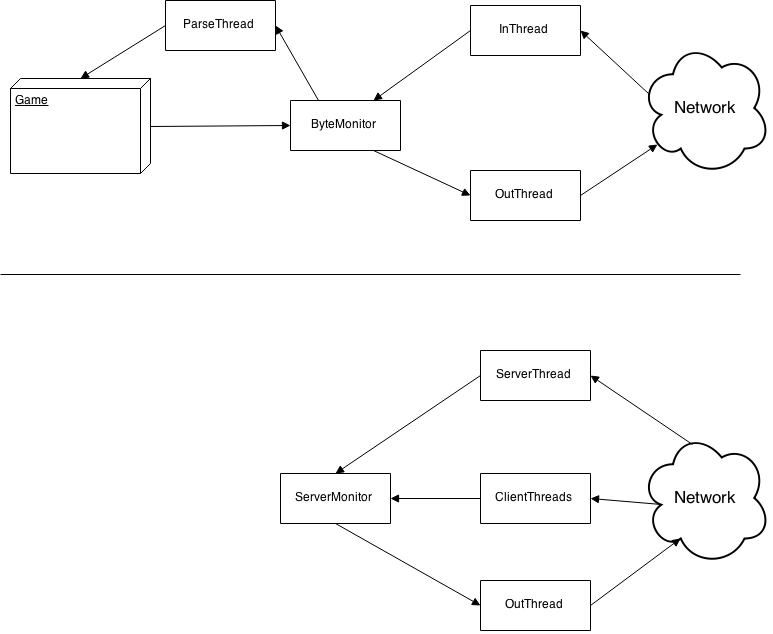
\includegraphics[width=0.8\textwidth]{spacedefence.png}
  \caption{Model of the network solution, first the client side, followed by the server.}
  \label{fig:network}
\end{figure}

The Server consists of:
\begin{itemize}
  \item Simple monitor with a message queue, and a set of connected clients.
  \item One InThread for each connected client that recieves messages and adds them to the message queue.
  \item One OutThread that reads messages from the queue and sends them to all clients.
\end{itemize}

The Client consists of:
\begin{itemize}
  \item A simple monitor that handles the byte message queues to and from the server.
  \item One InThread that reads messages from the server and adds them to a queue.
  \item One OutThread that reads messages from a queue and sends them to the server.
  \item One ParseThread that reads the byte messages sent from the server and translates them into the correct game events according to our network protocol.
  \item A simple monitor that keeps track of the game events.
  \item The game reads from this monitor and acts accordingly, and upon local event, sends the correct byte message to the byte monitor.
\end{itemize}

\section{Manual}

SpaceDefence is a game where up to four players are able to play against each other. The objective is to be the last player standing. 
Each player has its own board where the creeps arrive at the top of the board and work their way down toward the player's base, located at the bottom of the board.
All players connected to the game are shown in their own respective boards with their own creeps.
The gameplay mainly consists of defending one's own home base from the invading creeps. 
If creeps reach player home base, the player's hp is decreased. 
Collision with a creep results in player not being able to fire, but no decrease in hp. 
There is also a strategic element to it. 
A player has a steady income rate. Furthermore, credits are earned for each creep killed. 
One has to choose whether to spend credits on upgrading one's own ship or buy creeps to send to all other players. 
Upgrading the ship results in greater fire speed and increasing the passive income rate.
On the other hand, buying and sending creeps to the other players might overwhelm them resulting in creeps reaching their home base. Also, the income rate is increased when buying creeps. 

\subsection{Controls}

Each player controls its own ship. 
To move the ship the direction keys left and right is used. The movements is limited to each players own board.

To shoot, the space key is pressed. This shoots a bullet that may kill creeps.
Bullets can only be fired with a set fire rate. This depends on the players current level.

To upgrade the ship (fire rate and income rate) the z-key is pressed. 
This is only possible when enough credits has been collected.

To send creeps to the opponents the 1, 2, 3 keys are used.
1 sends one creep, 2 sends five creeps and 3 sends ten creeps to all connected opponents.

\subsection{Running the program}

The program consists of one server and one client part. 
The usual use case is that the player starting the client and initiating the game also starts up the server. The server is automatically started in conjunction with a \lq new game\rq but the server can also be started separately if needed.

When the program is downloaded from the website it consists of a compressed folder. 
Decompress it and go to the decompressed folder.
The decrompressed folder contains four .jar files. 
Three client jars which are platform dependent (Windows, OS X, Linux) and one for the server.

To start the server separately, start a terminal and write \texttt{java -jar server.jar}. 
When the server is started, the initiating player's ip is printed. This is used by the clients to connect to the server.
To start a client simply double click the provided client jar-file for your current platform. 
From within the client graphical user interface, a player starts a new game and, as previously stated, the server is started in conjunction with the said game.

\section{Evaluation}

By doing this project we have faced different challenges wihthin game development and network programming.
Overall the game came out some what as we expected. A lot of the techniques we have learnt during the labs 
have been useful during the project. We started by focusing on the network parts and thought it would be a fast job
and then we could focus on the game development. But it actually took more time than expected and althrough the project
there were network parts to fix or update. In the end we feel we have a good and robust solution. The solution works best
when using a wired network but works decent on wireless networks as well.

Developing the project have been a great experience to learn the practices of network programming in a fun and
relaxed context.

\section{Programs}
The source code can be found at:
\url{https://github.com/Jullekungfu/SpaceDefence}

For more info and downloadable jars please visit:
\url{http://jullekungfu.github.io/spacedefence}

\end{document}                 % The input file ends with this command.
